\documentclass[
12pt,
a4paper,
oneside,
headinclude,
footinclude]{article}

\usepackage[table,xcdraw,svgnames, dvipsnames]{xcolor}
\usepackage[capposition=bottom]{floatrow}
\usepackage[colorlinks]{hyperref} % to add hyperlinks
\usepackage{enumitem}
\usepackage{booktabs}
\usepackage{tabularx}
\usepackage{csquotes}
\usepackage{amsmath} % For the big bracket
\usepackage[export]{adjustbox}[2011/08/13]
\usepackage{array}
\usepackage{url}
\usepackage{graphicx} % to insert images
\usepackage{titlepic} % to insert image on front page
\usepackage{geometry} % to define margin
\usepackage{listings} % to add code
\usepackage{caption}
\usepackage[T1]{fontenc} % Use 8-bit encoding that has 256 glyphs
\usepackage[utf8]{inputenc} % Required for including letters with accents
\usepackage{color}
\usepackage{subcaption}
\usepackage[nochapters, dottedtoc]{classicthesis}
\usepackage{listings} % For Python code

\usepackage[ruled]{algorithm2e} % For pseudo-code

\usepackage{mathpazo}

\usepackage{lipsum} % For testing
\usepackage{color}

\usepackage{etoolbox}

\usepackage{tikz} % For trees plot
\usepackage{tikz-dependency} % For dependency graphs

\usepackage{bm} % For bold math

\usepackage{setspace}
\usepackage{minted}

% For tables
\usepackage{amssymb}

\definecolor{dkgreen}{rgb}{0,0.6,0}
\definecolor{gray}{rgb}{0.5,0.5,0.5}
\definecolor{mauve}{rgb}{0.58,0,0.82}

% ==== Define python syntax ====
\definecolor{Code}{rgb}{0,0,0}
\definecolor{Decorators}{rgb}{0.5,0.5,0.5}
\definecolor{Numbers}{rgb}{0.5,0,0}
\definecolor{MatchingBrackets}{rgb}{0.25,0.5,0.5}
\definecolor{Keywords}{rgb}{0,0,1}
\definecolor{self}{rgb}{0,0,0}
\definecolor{Strings}{rgb}{0,0.63,0}
\definecolor{Comments}{rgb}{0,0.63,1}
\definecolor{Backquotes}{rgb}{0,0,0}
\definecolor{Classname}{rgb}{0,0,0}
\definecolor{FunctionName}{rgb}{0,0,0}
\definecolor{Operators}{rgb}{0,0,0}
\definecolor{Background}{rgb}{0.98,0.98,0.98}
\lstdefinelanguage{Python}{
    numbers=left,
    numberstyle=\footnotesize,
    numbersep=1em,
    xleftmargin=1em,
    framextopmargin=2em,
    framexbottommargin=2em,
    showspaces=false,
    showtabs=false,
    showstringspaces=false,
    frame=l,
    tabsize=4,
    % Basic
    basicstyle=\ttfamily\small\setstretch{1},
    backgroundcolor=\color{Background},
    % Comments
    commentstyle=\color{Comments}\slshape,
    % Strings
    stringstyle=\color{Strings},
    morecomment=[s][\color{Strings}]{"""}{"""},
    morecomment=[s][\color{Strings}]{'''}{'''},
    % keywords
    morekeywords={import,from,class,def,for,while,if,is,in,elif,else,not,and,or,print,break,continue,return,True,False,None,access,as,,del,except,exec,finally,global,import,lambda,pass,print,raise,try,assert},
    keywordstyle={\color{Keywords}\bfseries},
    % additional keywords
    morekeywords={[2]@invariant,pylab,numpy,np,scipy},
    keywordstyle={[2]\color{Decorators}\slshape},
    emph={self},
    emphstyle={\color{self}\slshape},
    %
}


\lstset{language=Python}

\definecolor{webbrown}{rgb}{.6,0,0}

\usepackage{titlesec} % to customize titles
\titleformat{\chapter}{\normalfont\huge}{\textbf{\thechapter.}}{20pt}{\huge\textbf}[\vspace{2ex}\titlerule] % to customize chapter title aspect
\titleformat{\section} % to customize section titles
{\fontsize{14}{15}\bfseries}{\thesection}{1em}{}

\titlespacing*{\chapter}{0pt}{-50pt}{20pt} % to customize chapter title space

\graphicspath{ {../Figures/} } % images folder
\parindent0pt \parskip10pt % make block paragraphs
\geometry{verbose,tmargin=3cm,bmargin=3cm,lmargin=3cm,rmargin=3cm,headheight=3cm,headsep=3cm,footskip=1cm} % define margin
\hyphenation{Fortran hy-phen-ation}

\AtBeginDocument{%
    \hypersetup{
        colorlinks=true, breaklinks=true, bookmarks=true,
        urlcolor=webbrown, citecolor=Black, linkcolor=Black% Link colors
}}

\pagestyle{plain}
\title{\textbf{NLP Assignment 2: \\ Dependency Relations \&\\
        Transition-based Parser}}
\author{{Alberto Parravicini}}
\date{}	% default \today

% =============================================== BEGIN


\begin{document}
    \maketitle
    \pagenumbering{roman}
    \setcounter{page}{1}
    
    \section{Introduction}
    
    \begin{center}
        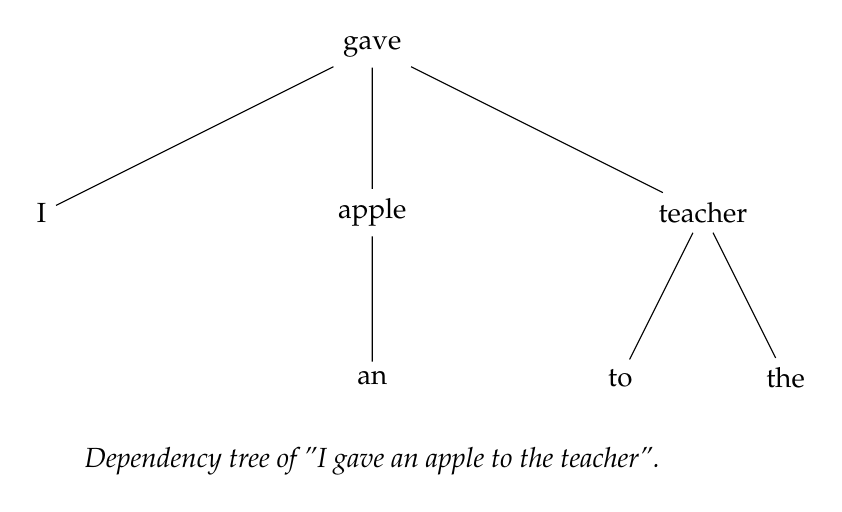
\begin{tikzpicture}[scale=1.4]
        \node (is-root) {gave}
        [sibling distance=3cm]
        child { node {I} }
        child {
            node {apple}
            [sibling distance=1.5cm]
            child { node {an} }
        }
        child { node {teacher}
            [sibling distance=1.5cm]
            child { node {to} }
            child { node {the} }
        };
        \path (is-root) +(0,-2.5\tikzleveldistance)
        node {\textit{Dependency tree of "I gave an apple to the teacher".}};
        \end{tikzpicture}
    \end{center}
   
    \begin{center}
        \scalebox{1.1} {
        \begin{dependency}[theme = simple]
            \begin{deptext}[column sep=1em, row sep=0.5ex]
                I \& gave \& an \& apple \& to \& the \& teacher \\
                PRON \& VERB \& DET \& NOUN \& ADP \& DET \& NOUN \\
            \end{deptext}
            \deproot{2}{ROOT}
            \depedge{2}{1}{NSUBJ}
            %\depedge[edge start x offset=-6pt]{2}{5}{ATT}
            \depedge{2}{4}{OBJ}
            \depedge[edge start x offset=-1pt]{4}{3}{DET}
            \depedge{2}{7}{OBL}
            \depedge{7}{5}{CASE}
            \depedge[edge start x offset=-5pt]{7}{6}{DET}
            %\depedge[arc angle=50]{7}{6}{ATT}
        \end{dependency}
        }
    \end{center}

    \begin{center}
        \begin{table}[H]   
            \hspace*{-2.0cm}
            \begin{tabular}{l p{5cm} p{5cm} l l} % creating eight columns
                \hline
                \hline 
                \\[-1.5ex]
                \textcolor{BrickRed}{Step} & \textcolor{BrickRed}{Stack} & \textcolor{BrickRed}{Buffer} & \textcolor{BrickRed}{Action} & \textcolor{BrickRed}{Output}\\ [0.5ex]
                \hline % inserts single-line
                \\[-1.5ex]
                0 & [\_\_ROOT\_\_] & [I, gave, an, apple, to, the, teacher] & SHIFT & \\ 
                1 & [\_\_ROOT\_\_, I] & [gave, an, apple, to, the, teacher] & SHIFT & \\ 
                2 & [\_\_ROOT\_\_, I, gave] & [an, apple, to, the, teacher] & LEFT & ( I $\rightarrow$ gave )\\ 
                3 & [\_\_ROOT\_\_, gave] & [an, apple, to, the, teacher] & SHIFT & \\ 
                4 & [\_\_ROOT\_\_, gave, an] & [apple, to, the, teacher] & SHIFT & \\ 
                5 & [\_\_ROOT\_\_, gave, an, apple] & [to, the, teacher] & LEFT & ( an $\leftarrow$ apple )\\ 
                6 & [\_\_ROOT\_\_, gave, apple] & [to, the, teacher] & RIGHT & ( gave $\rightarrow$ apple )\\ 
                7 & [\_\_ROOT\_\_, gave] & [to, the, teacher] & SHIFT & \\ 
                8 & [\_\_ROOT\_\_, gave, to] & [the, teacher] & SHIFT & \\ 
                9 & [\_\_ROOT\_\_, gave, to, the] & [teacher] & SHIFT & \\ 
                10 & [\_\_ROOT\_\_, gave, to, the, teacher] & [] & LEFT & ( the $\leftarrow$ teacher )\\ 
                11 & [\_\_ROOT\_\_, gave, to, teacher] & [] & LEFT & ( to $\leftarrow$ teacher )\\ 
                12 & [\_\_ROOT\_\_, gave, teacher] & [] & RIGHT & ( gave $\rightarrow$ teacher )\\ 
                13 & [\_\_ROOT\_\_, gave] & [] & RIGHT & ( \_\_ROOT\_\_ $\rightarrow$ gave )\\ 
                14 & [\_\_ROOT\_\_] & [] & DONE &                 
                \\[1ex] % [1ex] adds vertical space
                \hline % inserts single-line
            \end{tabular}
            \caption{\label{tab:trace-1}Execution trace for \textit{I gave an apple to the teacher}.}
        \end{table} 
    \end{center}

    \begin{center}
    \begin{table}[H]   
        \hspace*{-2.0cm}
        \begin{tabular}{l p{5cm} p{5cm} l l} % creating eight columns
            \hline
            \hline 
            \\[-1.5ex]
            \textcolor{BrickRed}{Step} & \textcolor{BrickRed}{Stack} & \textcolor{BrickRed}{Buffer} & \textcolor{BrickRed}{Action} & \textcolor{BrickRed}{Output}\\ [0.5ex]
            \hline % inserts single-line
            \\[-1.5ex]
            0 & [\_\_ROOT\_\_] & [Mary, missed, her, train, to, work] & SHIFT & \\ 
            1 & [\_\_ROOT\_\_, Mary] & [missed, her, train, to, work] & SHIFT & \\ 
            2 & [\_\_ROOT\_\_, Mary, missed] & [her, train, to, work] & LEFT & ( Mary $\leftarrow$ missed )\\ 
            3 & [\_\_ROOT\_\_, missed] & [her, train, to, work] & SHIFT & \\ 
            4 & [\_\_ROOT\_\_, missed, her] & [train, to, work] & SHIFT & \\ 
            5 & [\_\_ROOT\_\_, missed, her, train] & [to, work] & LEFT & ( her $\leftarrow$ train )\\ 
            6 & [\_\_ROOT\_\_, missed, train] & [to, work] & RIGHT & ( missed $\rightarrow$ train )\\ 
            7 & [\_\_ROOT\_\_, missed] & [to, work] & SHIFT & \\ 
            8 & [\_\_ROOT\_\_, missed, to] & [work] & SHIFT & \\ 
            9 & [\_\_ROOT\_\_, missed, to, work] & [] & LEFT & ( to $\leftarrow$ work )\\ 
            10 & [\_\_ROOT\_\_, missed, work] & [] & RIGHT & ( missed $\rightarrow$ work )\\ 
            11 & [\_\_ROOT\_\_, missed] & [] & RIGHT & ( \_\_ROOT\_\_ $\rightarrow$ missed )\\ 
            12 & [\_\_ROOT\_\_] & [] & DONE &             
            \\[1ex] % [1ex] adds vertical space
            \hline % inserts single-line
        \end{tabular}
        \caption{\label{tab:trace-2}Execution trace for \textit{Mary missed her train to work}.}
    \end{table} 
    \end{center}


    \begin{center}
    \begin{table}[H]   
        \hspace*{-2.0cm}
        \begin{tabular}{l p{5cm} p{5cm} l l} % creating eight columns
            \hline
            \hline 
            \\[-1.5ex]
            \textcolor{BrickRed}{Step} & \textcolor{BrickRed}{Stack} & \textcolor{BrickRed}{Buffer} & \textcolor{BrickRed}{Action} & \textcolor{BrickRed}{Output}\\ [0.5ex]
            \hline % inserts single-line
            \\[-1.5ex]
            0 & [\_\_ROOT\_\_] & [John, gave, the, teacher, a, very, heavy, book] & SHIFT & \\ 
            1 & [\_\_ROOT\_\_, John] & [gave, the, teacher, a, very, heavy, book] & SHIFT & \\ 
            2 & [\_\_ROOT\_\_, John, gave] & [the, teacher, a, very, heavy, book] & LEFT & ( John $\leftarrow$ gave )\\ 
            3 & [\_\_ROOT\_\_, gave] & [the, teacher, a, very, heavy, book] & SHIFT & \\ 
            4 & [\_\_ROOT\_\_, gave, the] & [teacher, a, very, heavy, book] & SHIFT & \\ 
            5 & [\_\_ROOT\_\_, gave, the, teacher] & [a, very, heavy, book] & LEFT & ( the $\leftarrow$ teacher )\\ 
            6 & [\_\_ROOT\_\_, gave, teacher] & [a, very, heavy, book] & RIGHT & ( gave $\rightarrow$ teacher )\\ 
            7 & [\_\_ROOT\_\_, gave] & [a, very, heavy, book] & SHIFT & \\ 
            8 & [\_\_ROOT\_\_, gave, a] & [very, heavy, book] & SHIFT & \\ 
            9 & [\_\_ROOT\_\_, gave, a, very] & [heavy, book] & SHIFT & \\ 
            10 & [\_\_ROOT\_\_, gave, a, very, heavy] & [book] & LEFT & ( very $\leftarrow$ heavy )\\ 
            11 & [\_\_ROOT\_\_, gave, a, heavy] & [book] & SHIFT & \\ 
            12 & [\_\_ROOT\_\_, gave, a, heavy, book] & [] & LEFT & ( heavy $\leftarrow$ book )\\ 
            13 & [\_\_ROOT\_\_, gave, a, book] & [] & LEFT & ( a $\leftarrow$ book )\\ 
            14 & [\_\_ROOT\_\_, gave, book] & [] & RIGHT & ( gave $\rightarrow$ book )\\ 
            15 & [\_\_ROOT\_\_, gave] & [] & RIGHT & ( \_\_ROOT\_\_ $\rightarrow$ gave )\\ 
            16 & [\_\_ROOT\_\_] & [] & DONE &           
            \\[1ex] % [1ex] adds vertical space
            \hline % inserts single-line
        \end{tabular}
        \caption{\label{tab:trace-2}Execution trace for \textit{John gave the teacher a very heavy book}.}
    \end{table} 
    \end{center}
    
    
    \begin{center}
    \begin{table}[H]   
        \hspace*{-2.0cm}
        \begin{tabular}{l p{5cm} p{5cm} l l} % creating eight columns
            \hline
            \hline 
            \\[-1.5ex]
            \textcolor{BrickRed}{Step} & \textcolor{BrickRed}{Stack} & \textcolor{BrickRed}{Buffer} & \textcolor{BrickRed}{Action} & \textcolor{BrickRed}{Output}\\ [0.5ex]
            \hline % inserts single-line
            \\[-1.5ex]
            0 & [\_\_ROOT\_\_] & [The, sun, shines] & SHIFT & \\ 
            1 & [\_\_ROOT\_\_, The] & [sun, shines] & SHIFT & \\ 
            2 & [\_\_ROOT\_\_, The, sun] & [shines] & LEFT & ( The $\leftarrow$ sun )\\ 
            3 & [\_\_ROOT\_\_, sun] & [shines] & SHIFT & \\ 
            4 & [\_\_ROOT\_\_, sun, shines] & [] & LEFT & ( sun $\leftarrow$ shines )\\ 
            5 & [\_\_ROOT\_\_, shines] & [] & RIGHT & ( \_\_ROOT\_\_ $\rightarrow$ shines )\\ 
            6 & [\_\_ROOT\_\_] & [] & DONE &     
            \\[1ex] % [1ex] adds vertical space
            \hline % inserts single-line
        \end{tabular}
        \caption{\label{tab:trace-2}Execution trace for \textit{The sun shines}.}
    \end{table} 
    \end{center}
    
    \bibliographystyle{plainurl}
    \bibliography{bibliography}
    
\end{document}